\documentclass{article}
\usepackage{amsmath}
\usepackage{mathtools}
\usepackage{txfonts}
\usepackage[margin=0.5in]{geometry}
\usepackage{graphicx}
\usepackage{float}
\graphicspath{ {images/} }


\setlength{\parskip}{\baselineskip}%
\setlength{\parindent}{0pt}%

\title{STAT 672 Final Project}
\author{Daniel Hartig}


\begin{document}
\maketitle

\section{Introduction}

This experiment creates a method for estimating the ridership at a subway station based on demographic characteristics of the surrounding area. 

For test and training data, I select the subway systems of two similar cities: Boston and Chicago. Both cities have similar population density in their downtown areas as well as similiar sized subway systems: Boston has 112 stations and 241 million yearly riders, Chicago has 136 stations and 238 million yearly riders. In addition, these cities have similar external features which could affect subway ridership: both cities' subway systems are at least 100 years old and thus well established, and both cities have cold winters that affect people's willingness to walk. 

Using data available from online sources, I calculate various `features' of each subway station on the network, and then apply regression-based machine learning to determine relationships between the features and subway ridership. Since ridership numbers vary depending on the day of the week, I use average weekday subway ridership as my target values. To support this choice, I use schedule values averaged between the morning and evecompletely ning rush hours for each system to determine such characteristics as travel time between stations and frequency of trains at each station. 

\section{Data Sources}

\subsection{Zip Code Data}

The data for this project comes from the US Census Bureau and is available at \texttt{factfinder.census.gov}. Subway ridership during weekdays is driven primarily by working commuters. A quick look at ridership data for the two cities shows that the highest usage stations are located in the Central Business Districts of their cities. To reflect the importance of commuters, I select four basic data types: total population, number of households, total number of employees, and net pay of all employees. This includes two different statistics to measure where people live, and two others to measure where people work. 

In addition to the counts of the above data types for each zip code, each zip code has a land area. Dividing the counts by the land area yields a density. Each zip code has a geographical centroid associated with it; I use this to determine proximity to various subway stations. Finally, the Census Bureau has shapefiles that lay out the land-water boundary for each state. I use the shapefiles for Massachussets and Illinois to differentiate between land and water. With the exception of the shapefiles, the other data is stored in a database. The shapefiles are accessed separately.

\subsection{Subway Station Data}

For each subway station, I obtain geographical coordinates for that station and ridership data. The ridership data came from self-reported numbers released in annual reports from the subway's operating agency (Massachussets Bay Transportation Authority for Boston; Chicago Transit Authority for Chicago). I locate the geographical coordinates on Google maps and record them into data files. Also included is a parking flag. This boolean value is true if there is parking available at the station, as indicated by the respective transit authority, and false if there is no parking available.

\subsection{Estimates of Density}

For each station, I estimate the average density within 1 km of the station for each of the data types. I accomplished this in a two step process: first I identify the zip codes close enough to the station to be important for calculating its density, then I make a weighted average density where the weights were the inverse of the distance from the station to each zip code.

Zip codes have irregular shapes, and geographical data for them is given by centroid, so it is hard to determine exactly what portion of which zip codes are within a certain radius of a station. To estimate if a zip code was close enough, I use a two part filter. First, I want to see if the zip code was close enough and large enough to be within 1 km of the station. I calculate this by using the square root of that zip code's area plus the radius of the station's area of interest (1 km) as a `proximity statistic,' and then determine if this is less than 1/2 of the distance between station and the zip code's centroid. Second, I want to see if there are any other zip codes between the station and the zip code of interest. To calculate this, I project the vector connecting the station to the zip code of interest onto all other closer zip code's vectors. I use the maximum magnitude projection subtracted from the proximity statistic as a `blocking statistic' and determine if this is less than 1/3 of the distance between station and zip code. The factors 1/2 and 1/3 are determined experimentally by checking the results of this 'nearest zip code' algorithm against a map.

The results of this nearest zip code approximation are shown in tabular and map form (Figure 1) for Sullivan Square station in the Charlestown neighborhood in Boston.

\begin{center}
\begin{tabular}{ c c c c c c c }
\hline
Zip Code & Distance to Station & sqrt(area) + 1& Large and Close & Projection & sqrt(area) + 1 - Proj & Not Blocked \\
\hline
\bf{02145} & 1.35 & 2.90 & True & N/A & 1.90 & True \\
\bf{02129} & 1.36 & 2.87 & True & -1.30 & 3.17 & True \\
\bf{02141} & 1.59 & 2.29 & True & 0.11 & 1.18 & True \\
\bf{02143} & 1.64 & 3.00 & True & 1.05 & 0.95 & True \\
02114 & 2.41 & 2.08 & True & 2.02 & -0.94 & False \\
02142 & 2.54 & 1.84 & True & 2.51 & -1.67 & False \\
\bf{02149} & 3.05 & 2.98 & True & 0.85 & 2.13 & True \\
02108 & 3.08 & 1.46 & False & N/A & N/A & N/A \\ 
02139 & 3.18 & 3.00 & True & 2.86 & 0.14 & False \\
\hline
\end{tabular}
\end{center}

\begin{figure}[H]\label{fig:f1}
\begin{center}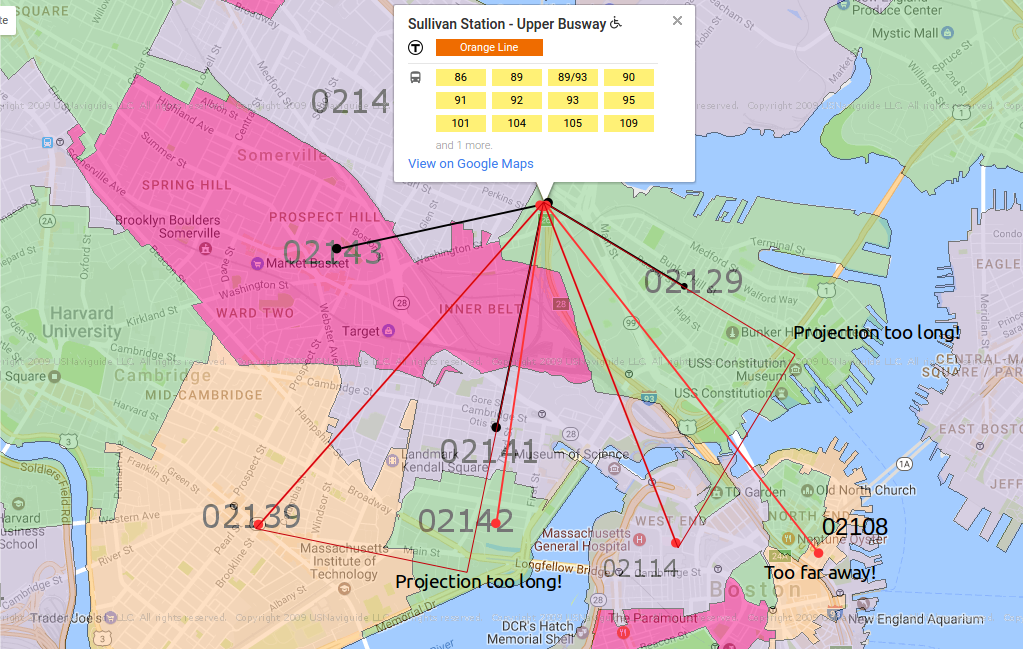
\includegraphics[scale=0.6]{Sullivan_for_distance_with_markup}\end{center}\caption{Illustration of nearst zip code estimation.}
\end{figure}



We can see that five zip codes are accepted (02145, 02129, 02141, 02143, 02149; in bold). Several others (02114, 02142, 02139) are close enough and large enough to be considered, but they are `blocked' by a closer zip code. Zip code 02108 and other, farther away zip codes do not meet the close enough and large enough criteria, and so their projections are not calculated. 

The next step is to calculate the data density for the five selected nearby zipcodes and take the weighted average of them. 

\begin{center}
\begin{tabular}{ c c c c c }
\hline
Zipcode & Distance & Inverse Distance & Density & Weighted Density \\
\hline
02145 & 1.35 & 0.74 & 7036 & 5211 \\
02129 & 1.36 & 0.74 & 4707 & 3461 \\
02141 & 1.59 & 0.63 & 7186 & 4519 \\
02143 & 1.64 & 0.61 & 6156 & 3753 \\
02149 & 3.05 & 0.33 & 4682 & 1535 \\
\hline
&&3.04&&18479 \\

\end{tabular}
\end{center}

\begin{figure}[H]\label{fig:f2}
\begin{center}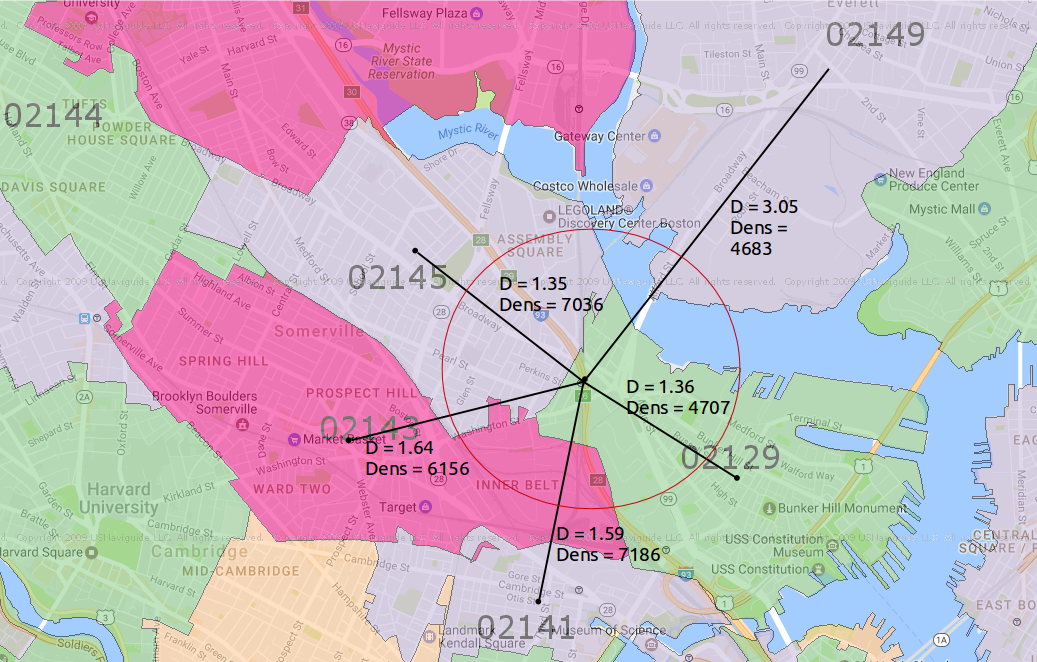
\includegraphics[scale=0.6]{Sullivan_for_density_with_markup}\end{center}
\caption{Illustration of density estimation.}\end{figure}

Dividing the summed weighted densities by the summed inverse distances yields a density estimate of 6074. While the estimate appears to be a good fit for the available data, the red circle at 1 km (Figure 2) shows the drawbacks of this method. While 02141's centroid is closer to Sullivan Station than 02143 is; because of the orientation of the two zip codes, the station's 1 km radius circle overlaps with 02143 but not 02141. 

\subsection{Estimates of Area}

I choose four different geographic interpretations of area for each of the four counting data types: the count within walking distance; the count within walking distance where the station of interest is nearest; the count within driving distance where the station of interest is nearest; and the count within walking distance of a certain minute ride from station of interest. 

To calculate walking distance, I assume that 1 km was the farthest from a station that a person is willing to walk. I then sample 10,000 points chosen randomly from a 1 km radius circle around the station. I compare these points against a shapefile of the state's geography to see if the points were on land or in water. The percentage of points found to be on land I multiplied by the area of the 1 km circle ($\pi$ km$^2$) to obtain the area within walking distance of each station. This will be referred to as the 'walking' data for a station.

To calculate the area that was both within walking distance and also closest to this station, I use a similar method. I sample the same 10,000 points within a 1 km circle, but in additon to checking against a shapefile to determine if the point was on land, I use a geographic r-tree index of stations to determine if any other station was closer to this point than the station of interest. The number of points that were both on land and closest to the station of interest is then divided by 10,000 and muliplied by the area of the walking distance circle to get the total area nearest to that station. This will be referred to as the 'nearest' data for this station.

This process is illustrated in Figure 3. The green dots are counted as good, while the red dots are closer to some other station and the blue dots are in the water. Out of 100 dots, 75 are green, 15 are red, and 10 are blue. The calulated `walking' area includes the green and red dots and represents 90\% of the area of the 1 km radius circle; the calculated 'nearest' area includes only the green dots and represents 75\% of the 1 km radius circle. 

\begin{figure}[H]\label{fig:f3}
\begin{center}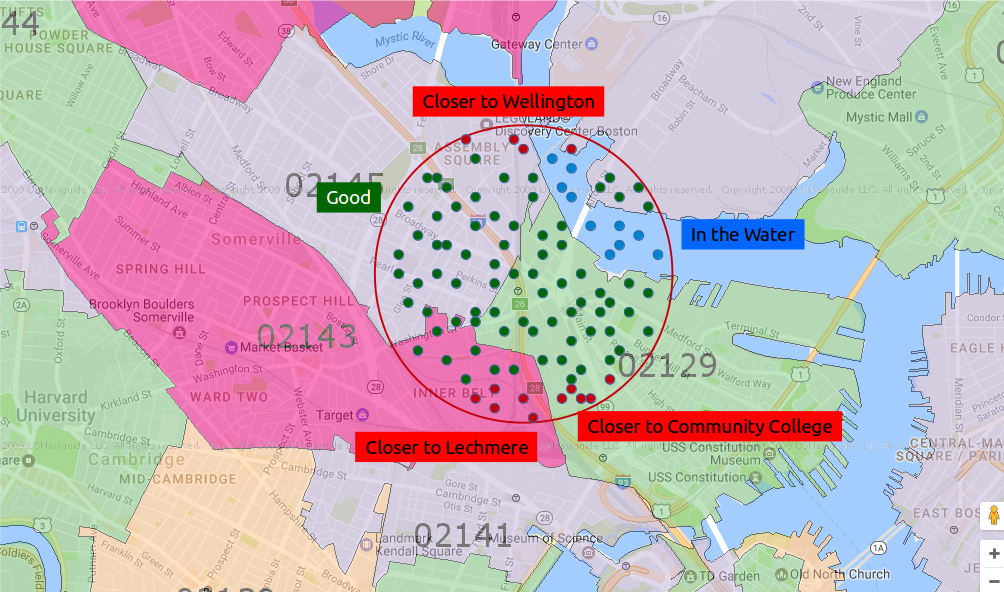
\includegraphics[scale=0.6]{area_with_markup}\end{center}
\caption{Illustration of determining area of a station.}
\end{figure}

For driving distance, I use a similar method but increase the radius of the circle to 15 km. I test points both to see if they are on land, and to see if they are closest to the station of interest.

The last geographic feature was determining the count within a 15 or 30 minute suway ride from this station. For this, I use scheduling data to build a graph of the entire subway system network. Each train line is represented by a series of interconnected nodes that can be traversed with a cost equal to the number of minutes in travel time between the two stations. For transfers between lines, I estimate the time cost to be half of the period of the line being transferred to. For example, if transferring from Boston's Orange Line to the Red Line at Downtown Crossing station, the Red line runs every 5 minutes during rush hour. Therefore a reasonable estimate of wait time in Downtown Crossing, if you arrived there at a random time, would be 2.5 minutes before a Red line train arrived. Thus the graph traversal cost from Downton Crossing's Orange line to Red line is 2.5 mintues. An example of pathing from Sullivan Square on the Orange line to South Station on the Red line is shown in Figure 4. 

\begin{figure}\label{fig:f4}
\begin{center}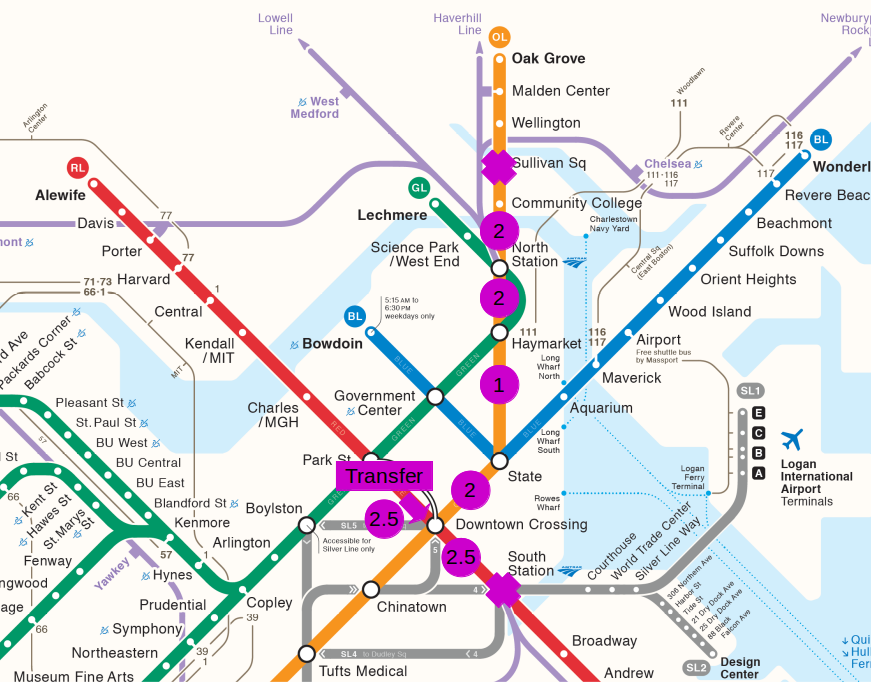
\includegraphics[scale=0.6]{transfer_with_markup}\end{center}
\caption{Determination of transit time from subway network graph.}
\end{figure}

Each interstation time is summed along with transfer times to get a total `distance' from Sullivan Square to South Station of 12 minutes. After building a graph of all such transit and transfer times, I find all stations that could be reached within 15 or 30 minutes from the station of interest. I then sum the `nearest' data for all those stations, to prevent overlapping data between stations. The result will be referred to as the `network' data for each station. 

\subsection{Station Data Estimates}

Putting all these factors together, I create data estimates for each station and for each area calculation. For every station on the network, I estimate the population, number of housholds, employment, and total pay for the area that is nearest to each station, within walking distance of each station, within  driving distance and nearest to each station, within a 15 minute transit trip from each station, and within a 30 mintue transit trip from each station. These 20 data points, along with the parking flag, comprise the feature set for this experiment.

\section{Regression}

Regression analysis is performed using the two cities as separate samples. Because the purpose of this experiement is to create a model that can be applied to a completely new city, it is important to consider each city on its own, as a complete network, without mixing the data set between cities. Therefore, for each regression method there are two pairs of training and test error, one for where Boston is the training set and Chicago the test set, and one with Chicago as the training set and Boston the test set. 

\subsection{Results}

\begin{center}\begin{tabular}{ c c c c c c}
\cline{3-6}
&&\multicolumn{2}{c}{Trn = Boston; Tst = Chicago}&\multicolumn{2}{c}{Trn = Chicago; Tst = Boston} \\ \hline
Test Type & Parameters & Training Error & Test Error &Training Error & Test Error \\
\hline\hline
Linear Least Squares & &0.721 & -0.557 & 0.685 & -1.778 \\
Linear SVR & C = 0.006& 0.526 & 0.207 & 0.343 & 0.207 \\
Ridge Regression & $\alpha$ = 350 &0.497 & 0.144 & 0.341 & 0.250 \\
LASSO Regression & $\alpha$ = 0.3&0.475 & 0.056 & 0.216 & 0.125 \\
Radial Basis Function SVR & C = 1.4, $\gamma$ = 0 &0.752& 0.135 & 0.730 & 0.223 \\
Polynomial SVR & C = 0.14, deg = 3& 0.547 & 0.506 & 0.760 & 0.117 \\
Sigmoid SVR & C = 0.08, $\gamma$ = 0& 0.404 & 0.125 & 0.134 & 0.183 \\
\end{tabular}\end{center}

\subsection{Discussion of methods}

The linear least squares classifier is standard linear regression using a least squares loss fuction. It has good performance in the training sets but is non-predictive on the test sets. The negative error indicates that predicting all stations to have ridership equal to mean ridership would have given better results.

For the remaining linear regression methods, a grid search is used to optimize the $C$ or $\alpha$ value for each method. Support Vector Regression with the linear kernel has moderate performance on the training sets but the best worst-case performance on the two test sets. Ridge regression performs almost as well as Linear SVR. LASSO regression peforms poorly by comparison to the previous two methods.

Among the non-linear regression kernels performed for comparison, the Radial Basis Function, using kernel function $\exp\left(-\gamma\left|x-x^\prime\right|^2\right)$, performs similarly on test errors as Linear SVR and Ridge Regression, but much better on the Training sets. Overall, this may be the best classifier. Polynomial SVR, using a 3rd degree polynomial kernel, is also interesting because of its widely divergent results between the two training sets. When Boston is used as the training set, the training error is mediocre, but test error is the best of any test. When Chicago is used as the training set, training error is the best of any test, but test error is mediocre. Sigmoid SVR, using the kernel function $\tanh\left(\gamma\left<x, x^\prime\right>\right)$, performs poorly compared to all other methods. 

\subsection{Discussion of Support Vector Regression}

In Support Vector Classification, the primal soft-margin problem is given by 

\begin{align*}
\min_{w_0\in\mathbb{R}, w\in\mathbb{R}^D, \xi\in\mathbb{R}^n}\frac{1}{2}\left\lVert w\right\rVert_2^2 + &\frac{C}{n}\sum_{i=1}^n\xi_i& \\ 
\text{subject to }&Y_i\left(w_0 + \left<w,\Phi(X_i)\right>\right) \geq 1 - \xi_i, \\
&\xi_i\geq 0, i = 1, ..., n
\end{align*}
with its dual optimization problem
\begin{align*}
\max_{\alpha\in\mathbb{R}^n}\sum_{i=1}^n\alpha_i - \frac{1}{n}\sum_{i=1}^n\sum_{j=1}^n&\alpha_i\alpha_jY_iY_j\left<\Phi(X_i), \Phi(X_j)\right> \\
\text{subject to }&\sum_{i=1}^n\alpha_iY_i=0 \\
&0 \leq \alpha_i \leq \frac{C}{n}, i=1, ... , n.
\end{align*}

The regression problem does not want to determine the sign, as the classifier does. Instead, it must predict a value so classification must success is achieved when the predicted value is closest to the actual values. Therefore, we introduce a parameter $\epsilon$ that represents the error threshold, beyond which a data point will be penalized proportional to C. 

In Support Vector Classification, the slack variables ($\xi_i$) have a non-negativity constraint, and there is one type of classification error, misclassification. However, in regression, there are two types of `misclassification' to be avoided, overestimation and underestimation. Therefore, two slack variables are required with the non-negativity constraint ($\xi_i, \xi_i^*$).

Therefore, the primal problem for Support Vector Regression is given by 
\begin{align*}
\min_{w_0\in\mathbb{R}, w\in\mathbb{R}^D, \xi,\xi^*\in\mathbb{R}^n}\frac{1}{2}\left\lVert w\right\rVert_2^2 + &\frac{C}{n}\sum_{i=1}^n\left(\xi_i+\xi_i^*\right)& \\ 
\text{subject to }&Y_i-w_0 - \left<w,\Phi(X_i)\right> \leq \epsilon + \xi_i, \\
&-Y_i+w_0 + \left<w,\Phi(X_i)\right> \leq \epsilon + \xi_i^*, \\
&\xi_i, \xi_i^*\geq 0, i = 1, ..., n
\end{align*}
with its dual optimization problem
\begin{align*}
\max_{\alpha, \alpha^*\in\mathbb{R}^n}\sum_{i=1}^nY_i\left(\alpha_i-\alpha^*_i\right) - \frac{1}{n}\sum_{i=1}^n\sum_{j=1}^n&\left<\alpha_i-\alpha_i^*, \alpha_j-\alpha_j^*\right>\left<\Phi(X_i), \Phi(X_j)\right> - \epsilon\sum_{i=1}^n\alpha_i+\alpha^*_i\\
\text{subject to }&\sum_{i=1}^n\alpha_i-\alpha_i=0 \\
&0 \leq \alpha_i, \alpha_i^* \leq C, i=1, ... , n.
\end{align*}

\section{Error Analysis}

No regression methods are very effective for making predictions about the subway ridership in the test set. Among the linear methods, the best predictivity belongs to Linear SVR; but the ratio of explained variation to total variation is still only about 20\%. Therefore we must make some efforts to determine the source of this error and determine if there are methods we can use to abate the error in future iterations of this experiment. 

\subsection{Linear Coefficient Analysis}

An advantage of comparing linear regression methods is that there exists a medium for direct comparison. The feature coefficients of each regression, when run on standardized data, are directly comparable to each other. Therefore, for each of the features in our feature set, we can plot the coefficients obtained in various methods.

\begin{figure}[H]\label{fig:f5}
\begin{center}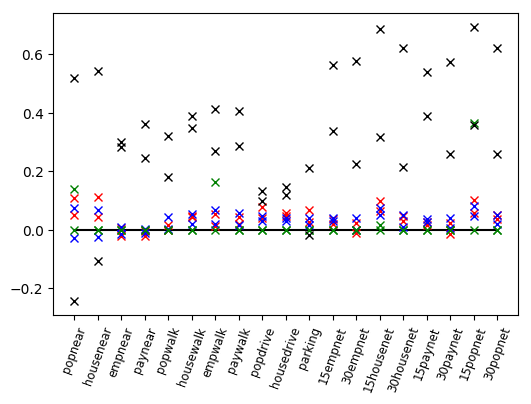
\includegraphics[scale=1]{coef_by_type}\end{center}
\caption{Feature name vs. linear coefficient. Least squares in black, SVR in red, Ridge in blue, LASSO in green.}
\end{figure}

In the plotted graph in Figure 5, we see that the three more advanced methods produce relatively well clustered coefficients, while the coefficients for linear regression vary considerably.

\pagebreak
We also see that some coeffients are more useful than others. Coefficients with a tight cluster are more likely to be accurate. However, if that tight cluster is around 0, then this indicates that this coefficient is not an effective predictor. For example, both `empnear' and `paynear' are tightly clustered around zero, indicating that those feature have no predictive value. The `popnear' feature, on the other hand, attains some high values, but has a wide spread of both postiive and negative coefficients, casting doubt on its predictive value as well. For `15popnet', the cluster is not very tight, but it is clearly positive, indicating this may be a valuable feature.

\begin{figure}[H]\label{fig:f6}
\begin{center}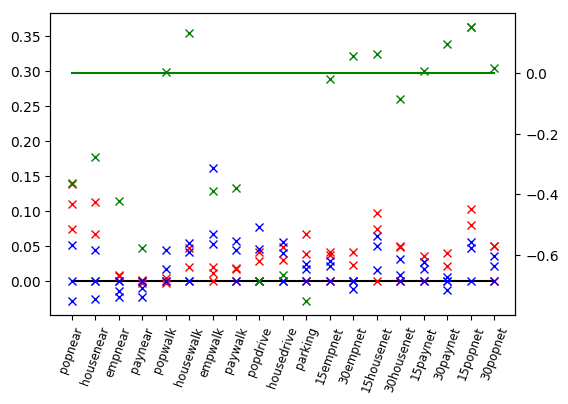
\includegraphics[scale=1]{coef_by_city}\end{center}
\caption{Feature name vs. linear coefficient and error. Chicago in blue, Boston in red, error in green.}
\end{figure}

For analyzing the spread of the coefficients, it is important to know the city which was used to fit the data since it is possible that the coefficients are different between the two cities. We can see this analysis in Figure 6. There are indeed some significant differences between the cities regarding the coefficients of some of the features. For example, 'empwalk' has a strong positive correlation with subway ridership in Chicago, but much less so in Boston. The feature 'popnear' is the opposite, with a strong correlation with subway ridership in Boston, but a neutral or negative relationship in Chicago. 

Correspondingly, we can see that for both of these features the error is highly negative. The error was calculated from a single-feature least squares regression, fit on one city and tested on the other. The errors from both cities as the training data are then averaged to get the error score shown. Negative values for the error mean that the coefficient for this feature trained on one city may have an opposite sloped linear relationship with subway ridership in the other city.

Going forward, it will be important to find a way to predict which features will not have a consistent relationship with ridership between cities. Also, it is interesting to note that all of 'empnear', 'paynear', 'empwalk' and 'paywalk' have strongly negative error scores. Since these are the four features that measure employment in the vicinity of the subway station, this implies that Boston and Chicago have significantly different relationships between employment and subway ridership. It may imply that subway traffic is primarily driven by high employment areas in one system, but not the other. 


\subsection{Outlier Analysis}

In addition to breaking down the error by feature, we can attempt to break down error by subway station. For both training sets, we can fit the model and then plot the actual ridership values against the predicted values. We can then determine if there is a relationship between error and actual subway ridership. 

\begin{figure}[H]\label{fig:f7}
\begin{center}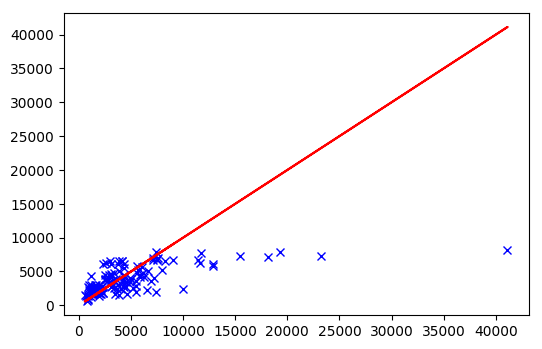
\includegraphics[scale=1]{actual_vs_predicted_chi}\end{center}
\caption{Actual ridership values on the x-axis, predicted values from Linear SVR on the y-axis.}
\end{figure}

The diagram in Figure 7 makes it painfully obvious that there is such a relationship. In the case of Chicago, the SVR model conservatively does not predict higher ridership scores at all. It does correctly predict the highest ridership station: the State-Lake-Washington joint station is the busiest in the city, by a large margin. However, where it attracts around 41,000 riders per day, the model only predicts 8,000 riders. 

\begin{figure}[H]\label{fig:f8}
\begin{center}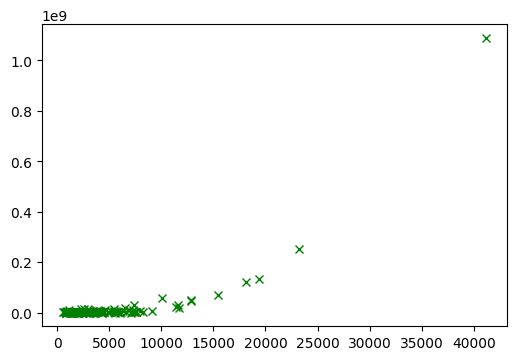
\includegraphics[scale=1]{actual_vs_error_chi}\end{center}
\caption{Actual ridership values on the x-axis, prediction error for Linear SVR on the y-axis}
\end{figure}

Plotting error against actual ridership makes the source of error in the SVR model even more obvious. As seen in Figure 8, 45\% of the total error in the model is attributable to a single data point: the State-Lake-Washington station. The next four stations (Washington Library-Jackson, Clark-Lake, Monroe, and Chicago-Red line) by error are also the next four stations by actual ridership, and four of the next five predicted riderships as well; the model is doing a good job! However, since the model is restricted to linear estimates, the error for these stations is very high as well. The five mentioned stations, all within a 1 km radius in Downtown Chicago, account for 75\% of the error in the model.

It is important to know that while the model is doing a good job in ranking the stations in order of ridership, it is not doing good job in predicting actual ridership. The clear resolution is that the model needs some non-linear components to be able to account for dramatically increased ridership in downtown areas. Chicago has a very centralized and concentrated job distribution. According to the American Factfinder, there are about 930,000 jobs in Chicago, over an area of 589 km$^2$. However, 330,000 of those jobs, over a third, are located in just 2.5 km$^2$ of downtown. A linear model will not be able to account for this disparity in job concentration. 



\subsection{Data Deficiencies}
The data and graphs for Boston show a similar story regarding increased error with ridership; though not quite as extreme as Chicago, since Boston's employment is not as concentrated. However, looking at the highest error stations, some other deficiencies become apparent. These deficiencies are not so much in the model as in the data underlying the model.

Boston is built on a series of peninsulas, unlike Chicago. Chicago does have a narrow river in its downtown, but Boston has the wider Charles River, several other smaller rivers, and Boston Harbor. Importantly, dense parts of the metroplitan area such as the Logan Airport, Charlestown and Cambridge are across bodies of water from the downtown. This makes it particularly important to properly account for water locations when gathering data. 

As opposed to Chicago where all the highest errors occured from underestimating ridership in the downtown, there are several stations near downtown Boston where predicted ridership is too high. Aquarium station has the second highest predicted ridership at 10971, but actual ridership is 49th at 4776. Bowdoin and Science Park have similarly high predcited ridership (7366 and 6822, respectively) and low actual riderships (1526 and 1042). 

\begin{figure}[H]\label{fig:f9}
\begin{center}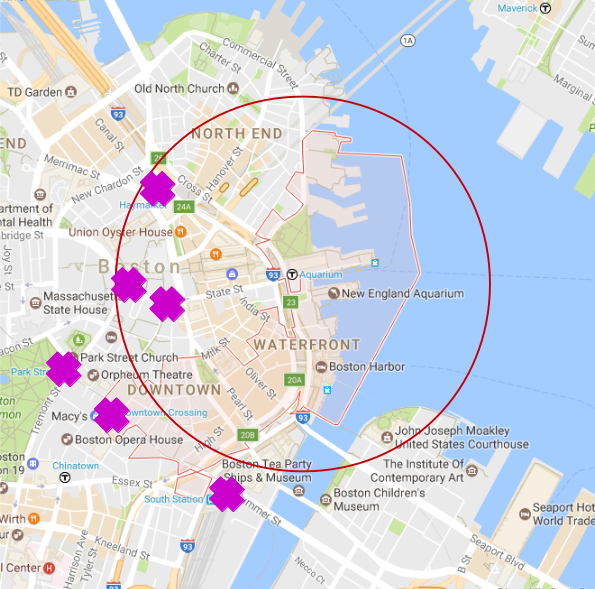
\includegraphics[scale=0.6]{Aquarium_with_markup}\end{center}
\caption{Illustration of Aquarium station, with other stations marked in pink and 1 km radius in red}
\end{figure}

An explanation can be found in Figure 9. For reasons that are not clear, the Census Bureau's shapefiles for Boston Harbor include much of the Harbor as land area. Google Map's zip code images, which follow the Census shapefiles, can be used to illustrate the problem. When the area determining algorithm generates random points within 1 km of Aquarium station, many points that should be in the Harbor are counted on land. Aquarium should have a relatively small nearby area, since it is hemmed in by the water and many other stations in the Downtown. However, its area is much larger than it should be because of the improperly counted Harbor area. As a result, Aquarium's high employment density is multiplied by an area too large by a factor of about 4. Therefore, Aquarium has the highest estimated nearby employment of any station; this is not a good estimate. We can see from this analysis that accuracy in the stations around downtown Boston will be limited until we can find a better way to determine land versus water in Boston Harbor.


\section{Conclusions and Further Work}

The models presented in this experiment were able to produce useful information regarding the relationships between subway ridership and the demographics of the areas. However, there are several hurdles that need to be over come to make the models more accurate.

The first hurdle is improving the quality of the data. The estimates of density are generally acceptable, but they could be improved with higher resolution source data. The most apparent improvement would be from getting higher resolution shapefiles of shorelines to determine whether points were on land or sea. In addition, in the dense Central Business Districts of major cities, the method of calculating the 'nearest' station doesn't always make sense. At some locations, there can be up to five subways stations within 0.5 km of a single point. A person's choice of station at which to catch a train may depend on things other than strict proximity. Some research is required to determine what other factors may be important.

Another hurdle is the presence of outliers. The stations of the Central Business Districts have far higher job densities than the median station, by a factor of 20 in Boston, and up to 40 in Chicago. We noted both that the models were very bad at predicting the higher ridership of these stations, and that the correlation coefficients for employment related factors were very close to zero. This implies that the relationship between employment and ridership is non-linear. This relationship should be more fully explored and the models adjusted accordingly.

Finally, several coefficients differ in magnitude and even sign between the two cities in our sample. More research is required to determine if there is any sort of relationship between these features and ridership. One possibility is to calculate coefficients and errors for all of the first order products of features. Another possibility is to use a third dataset to see if there are other clusters of coefficients can be found. Washington DC is the third subway system in the United States of roughly equal size to Boston and Chicago, with 234 million riders and 91 stations (compare to statistics in the Introduction).

In all, there are a variety of ways to improve the model and further determine the root causes of model performance and failure. 






 






\end{document}